\section{Algorithm through Linked List Examples}
A {\tt List} ADT in the
\SpecL{} program is defined at line {\tt A0}
in \cref{fig:llAllocSpec}. An empty list is represented
by the
constant {\tt LNil()}\footnote{{\tt LNil()} represents the application
of the nullary constructor {\tt LNil} on the unit value {\tt ()}. For brevity,
we will simply write {\tt LNil} for {\tt LNil()} henceforth.};
a non-empty list uses
the {\tt LCons} constructor to combine its first value ({\tt val:i32})
and the remaining list ({\tt tail:List}).
\SpecL{} supports
{\tt i<N>} (bitvectors of length {\tt N}),
{\tt bool}, and {\tt unit} types, also called {\em scalar types}.
\SpecL{}'s type system prevents
the creation of cycles in ADT values.
If {\tt l} is
an object of type {\tt List}, then to access its
constituent values, we may expand (or unroll) {\tt l} to
\begin{small}
\begin{equation}\label{eqn:specDeconstruct}
U_S: {\tt l\ =\ \underline{if}\ l}\ \ is\ \ {\tt LNil\ \ \underline{then}\ \ LNil\ \ \underline{else}\ \ LCons(l.val,l.tail)}
\end{equation}
\end{small}
In this expanded representation of {\tt l},
the {\em sum-deconstruction} operator\footnote{The sum-deconstruction operator `\sumDtor{}' for a sum type $T$ must contain exactly one branch for each top-level value constructor of $T$.
For example, `\sumDtor{}' for the {\tt List} type must have exactly two branches of the form {\tt LNil} and {\tt LCons}($e_1$,$e_2$) for some expressions $e_1$ and $e_2$.}
`\sumDtor{}'
deconstructs a sum type where the
\underline{if} condition `{\tt l} {\em is} {\tt Constructor}'
checks whether the top level constructor of {\tt l} is `{\tt Constructor}'.
If {\tt l}
is a non-empty list constructed through {\tt LCons},
then {\tt l.val} and {\tt l.tail}
are used to access {\tt l}'s first value and {\tt l}'s tail respectively.
The right-hand side of
\cref{eqn:specDeconstruct} can also be viewed as an executable
program that unrolls the input {\tt List} object {\tt l} once and
outputs a {\tt List} object constructed from {\tt l}'s constituents --- we
call \cref{eqn:specDeconstruct} the {\em unrolling procedure} $U_S$ of the {\tt List} ADT.
%We will later unify this expanded representation of a {\tt List} object with
%its C implementation.

\begin{figure}
\begin{tabular}{@{}c@{}c@{}}
\begin{subfigure}[b]{0.5\textwidth}
\begin{center}
{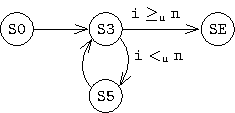
\includegraphics[scale=1.4]{chapters/figures/figMallocSpecCfg.pdf}}
\vspace{15pt}
\end{center}
\caption{\label{fig:llAllocSpecIRCFG}CFG of \SpecL{} program}
\end{subfigure}%
&
\begin{subfigure}[b]{0.5\textwidth}
\begin{center}
{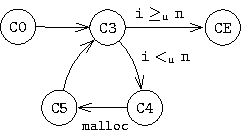
\includegraphics[scale=1.4]{chapters/figures/figMallocCCfg.pdf}}
\end{center}
\caption{\label{fig:llAllocCCFG}CFG of C program}
\end{subfigure}%
\\
\end{tabular}
\caption{\label{fig:mallocSpecCFGAndCCFG}CFG representation of Spec and C IRs shown in \cref{fig:llAllocSpecIR,fig:llAllocCIR} for the {\tt mk\_list} procedures in \cref{fig:llAllocSpec,fig:llAllocC} respectively.}
\end{figure}


\Cref{fig:llAllocSpecIRCFG,fig:llAllocCCFG} show the Control-Flow Graph (CFG) representations
of the \SpecL{} and C programs in \cref{fig:llAllocSpecIR,fig:llAllocCIR} respectively.
The CFG nodes represent PC locations of the program, and edges represent
transitions through instruction execution. For brevity, we sometimes represent
multiple program instructions with a single edge, e.g., in \cref{fig:llAllocCCFG}, the edge {\small \tt C5$\rightarrow$C3}
represents the path {\small \tt C5$\rightarrow$C6$\rightarrow$C7$\rightarrow$C8$\rightarrow$C3}. A control-flow edge is associated
with an {\em edge condition} (the condition under which that edge is taken),
a {\em transfer function} (how the program state is mutated if that edge is taken),
and a {\em UB assumption} (what condition should be true for the program
execution to be
well-defined across this edge). For example, the UB assumption associated with a division
instruction in $S$ will encode that the divisor must be non-zero.